\documentclass[ProofPDF]{./Styles/Jnls-Template-V3}

\begin{document}

\jname{Transactions of the International Society for Music Information Retrieval }
\jvol{00}
\jissue{00}
\jmonth{season}
\jyear{xxx}
\jid{doi}
\artid{xx.xxxx/xxxx.xx}
\filename{main}
\def\MSFirstPage{\pageref{startPage_Label}}
\def\MSLastPage{\pageref{endPage_Label}}
\graphicspath{{./figures/}}
\label{startPage_Label}
\title{Paper Template for TISMIR}

\articletype{RESEARCH ARTICLE}
% \articletype{DATASET ARTICLE}

\author[1]{Frédéric Chopin}
\howtociteauthor[1]{Frédéric Chopin}
\rhauthor[1]{F. Chopin}
\author[2]{Johann Sebastian Bach}
\howtociteauthor[2]{J. S. Bach}
\rhauthor[2]{J. S. Bach}

\aff[1]{Fryderyk Chopin Institute, Warsaw, Poland, \href{mailto:chopin@nifc.pl}{chopin@nifc.pl}}
\aff[2]{Bach Archive, Leipzip, Germany, \href{mailto:bach@bach-leipzig.de}{bach@bach-leipzig.de}}
\afflnote{*Author affiliations can be found in the back matter of this article}

\begin{history}
\submitted{\submittedday{xxx}\submittedmonth{xxx}\submittedyear{xxx}}
\accepted{\acceptedday{xxx}\acceptedmonth{xxx}\acceptedyear{xxx}}
\published{\publishedday{xxx}\publishedmonth{xxx}\publishedyear{xxx}}
\end{history}

\begin{abstract}[ABSTRACT]
Research articles must have the main text prefaced by an abstract of roughly 250 words summarising the main arguments and conclusions of the article.
This must have the heading ``Abstract'' and be easily identified from the start
of the main text.
\end{abstract}

\begin{keyword}[KEYWORDS:]

Transcription, classical music, machine learning

\end{keyword}

\maketitle

% comment out after review
\linenumbers

%%%%%%%%%%%%%%%%%%%%%%%%%%%%%%%%%%%%%%%%%%%%%%%%%%%%%%%%%%%%%%%%%%%%%%%%%%%%%%%%
% Main Content Start
%%%%%%%%%%%%%%%%%%%%%%%%%%%%%%%%%%%%%%%%%%%%%%%%%%%%%%%%%%%%%%%%%%%%%%%%%%%%%%%%
\section{Introduction}\label{sec:intro}

The Transactions of the International Society for Music Information Retrieval publishes novel scientific research in the field of music information retrieval (MIR), an interdisciplinary research area concerned with processing, analysing, organising and accessing music information. We welcome submissions from a wide range of disciplines, including computer science, musicology, cognitive science, library, and information science and electrical engineering.
Articles must not be longer than 8,000 words in length, including all referencing, citation, and notes.
Further information about the different article types and submission guidelines can be found online.\endnote{\url{https://transactions.ismir.net/about/submissions}}

Articles accepted for publication will be asked to pay an Article Publication Charge (APC) to cover publication costs. If you do not have funds available to pay the Article Publication Charge (APC) (e.g., because your institution/funder does not offer such support), you may request a waiver from ISMIR\endnote{\url{https://www.ismir.net}} to cover these costs. You can request a waiver at any stage during the editorial process, but it is best to raise this as early as possible - ideally including the request in your cover letter.

The funds are available to all submitting authors, but are intended to support those who do not have access to any funds to cover the APC. In your request, please outline in no more than 100 words why you require a waiver and a decision will be made by the Editors-in-Chief (EiC). Should you have any questions about this waiver option or the APC in general, please contact the EiC at your earliest convenience:



\section{Headings}\label{sec:headings}

Up to three level headings may be present and must be clearly identifiable
using different font sizes, bold or italics. If accepted for publication,
these will be converted into journal during typesetting.

As a general rule, submissions should be structured so that introduction,
methods, conclusions and discussion are all clearly indicated by a first level heading.

\subsection{Level heading 2}

\lipsum[66]

\subsubsection{Level heading 3}

\lipsum[75]

\section{Footnotes/Endnotes}\label{sec:footnotes}

Use endnotes (\verb=\endnote=) rather than footnotes
(we refer to these as ``Notes'' in the online publication).
These will appear at the end of the main text, before ``References''.
All notes should be used only where crucial clarifying information
needs to be conveyed.
Avoid using notes for purposes of referencing, with in-text citations used
instead.
If in-text citations cannot be used, a source can be cited as part of a note.
Please insert the endnote marker after the end punctuation.

\section{Figures}\label{sec:figures}

Figures must all be cited in the main text, in sequential order.
All figures should be placed within the text file upon submission and during
the review process. Figures/images have a resolution of at least 150 dpi
(300 dpi or above preferred). The files are in one of the following formats:
JPG, TIFF, GIF, PNG, EPS, PDF (to maximise quality,
the original source file is preferred).

After editorial acceptance, you will be asked to provide the figure
images in high resolution files, rather than in the submission file,
so that this quality is transferred into the publication.
The typesetting process will place the figures in an appropriate
location in the PDF.

Each figure must have an accompanying descriptive main title.
This should clearly and concisely summarise the content and/or
use of the figure image.
A short additional figure legend is optional to offer a further description.


% ------------------------------------------------------------
\begin{figure}[t]
  \centering
  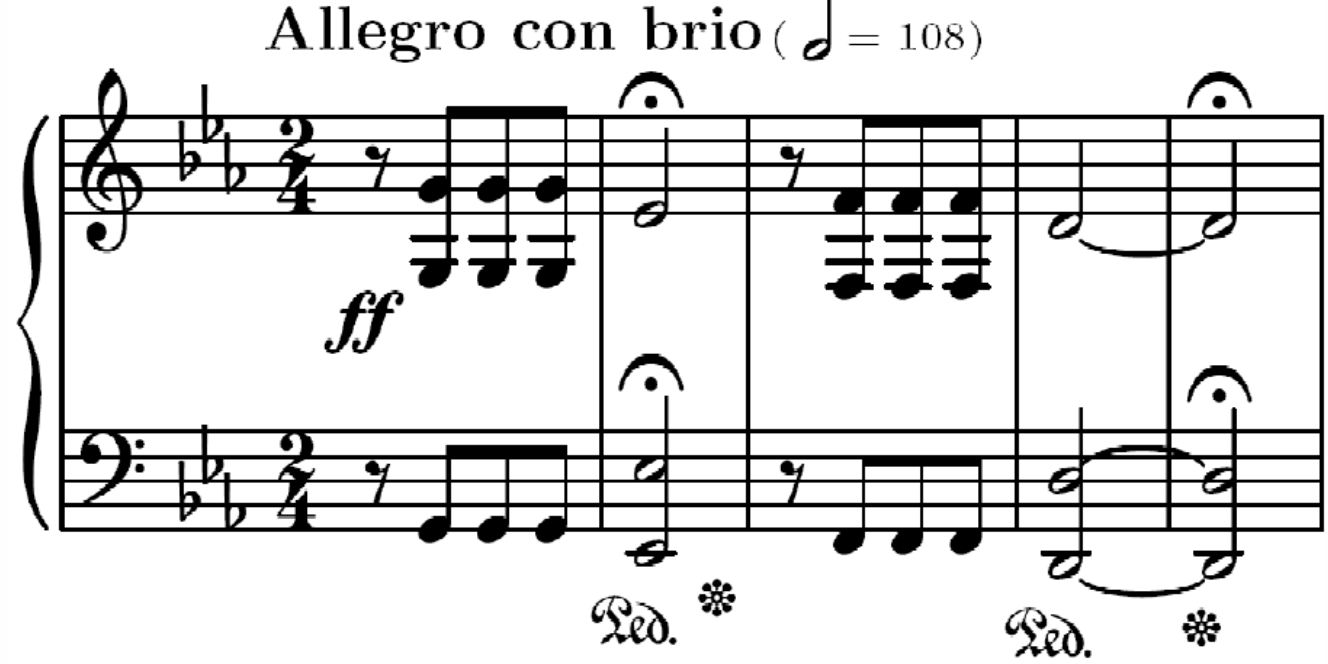
\includegraphics[width=0.85\columnwidth]{figures/figure_Beethoven.png}
  \caption{Figure captions should be descriptive and placed below the corresponding figure. Example caption: Sheet music representation of the first five measures of Symphony No. 5 by Ludwig van Beethoven in a piano-reduced version (reproduced from \cite{Mueller21_FMP_SPRINGER}, courtesy of the author).}
\label{fig:figure}
\end{figure}
% ------------------------------------------------------------

% ------------------------------------------------------------
\begin{figure*}[t]
  \centering
  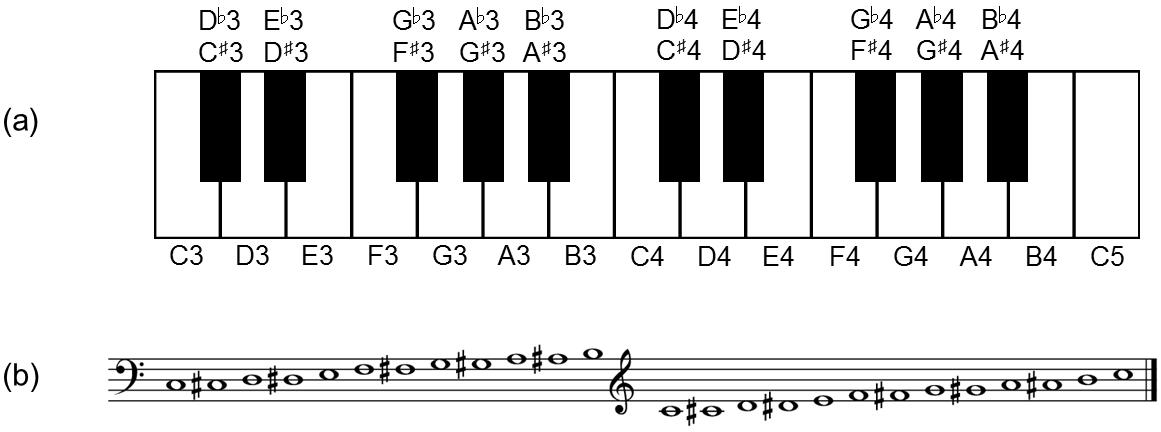
\includegraphics[width=12cm]{figures/figure_PianoKeys_ChromaticScale.png}
  \caption{Figures may span two columns and can consist of multiple parts labeled (a), (b), and so on. Note that the electronic (web) version of the article is displayed in a single-column format, which may significantly affect the figure size and layout. We therefore recommend preparing figures for the two-column format, as shown here, to ensure a clear and consistent appearance in both the PDF and web versions. Example caption: \textbf{(a)} Section of piano keyboard with keys ranging from C3 to C5. \textbf{(b)} Corresponding notes
using Western music notation.  (Reproduced from \cite{Mueller21_FMP_SPRINGER}, courtesy of the author.)}
\label{fig:figure_two_column}
\end{figure*}
% ------------------------------------------------------------

\section{Tables}\label{sec:tables}

Tables must be created using a word processor's table function,
not tabbed text.
Tables should be included in the manuscript.
The final layout will place the tables as close to their first
citation as possible.

All tables must be cited within the main text, numbered with Arabic
numerals in consecutive order (e.g., Table 1, Table 2, etc.).

Each table must have an accompanying descriptive title.
This should clearly and concisely summarise the content and/or
use of the table.
A short additional table legend is optional to offer a further
description of the table.

\subsection{Tables should not include}

\begin{itemize}
  \item Rotated text
  \item Colour to denote meaning (it will not display the same on all devices)
  \item Images
  \item Vertical or diagonal lines
  \item Multiple parts (e.g., ``Table 1a'' and ``Table 1b'').
  These should either be merged into one table,
  or separated into ``Table 1'' and ``Table 2''.
\end{itemize}

% ------------------------------------------------------------
\begin{table}[t]
    \centering
    \begin{tabular}{lc}
        \hline
        \colhead{Name} & \colhead{Period}\\
        \hline
        Medieval & ca. 500-1400\\
        Renaissance & ca. 1400-1600\\
        Baroque &  ca. 1600-1750\\
        Classical &  ca. 1730-1820\\
        Romantic &  ca. 1800-1910\\
        Modernism & from ca. 1890\\
        Contemporary & from ca. 1945\\
        \hline
    \end{tabular}
    \caption{Major eras of Western classical music.}\label{tab:table}
\end{table}
% ------------------------------------------------------------

\section{Equations}\label{sec:equations}

Equations should be placed on separate lines and numbered.
The number should be on the right side, in parentheses,
as in Eqn.~(\ref{eq:eq}).

\begin{align}\label{eq:eq}
E = mc^2
\end{align}

\section{Line numbers}
Line numbers are printed in the margins to facilitate the
review process. To remove line numbers for the camera-ready
version of your paper, comment \verb=\linenumbers= command
at the beginning of the document.

\section{Reproducibility (if applicable)}

If the content of your submission relates to data or software
that has been deposited in a code or preservation repository,
please provide summary information here, along with a DOI that
links to the deposited code/data.

\section{Competing interests}

If any of the authors have any competing interests then these
must be declared. A short paragraph should be placed before
the references.
Guidelines for competing interests are available online.%
\endnote{Link to guidelines: \\
  \url{http://transactions.ismir.net/information/competingInterestGuidelines}}


\section{Ethics and consent}

Research involving human subjects, human material, or human data,
must have been performed in accordance with the Declaration of Helsinki.
Where applicable, the studies must have been approved by an appropriate
ethics committee and the authors should include a statement within
the article text detailing this approval, including the name of the ethics committee and reference number of the approval.
The identity of the research subject should be anonymised whenever possible.
For research involving human subjects, informed consent to participate
in the study must be obtained from participants (or their legal guardian).
%
Experiments using animals must follow national standards of care.
For further information, click \href{http://bit.ly/1rBoe0S}{here}.


\section{References}

All citations must be listed at the end of the text file,
in alphabetical order of authors' surnames.
References should not be listed if they are not cited in
the main text.
This journal uses the APA system.
Please visit the journal's website
for examples of referencing format.\endnote{Link to citation examples: \\
\url{http://transactions.ismir.net/about/submissions/\#References}}

In this template, you can use \verb=\citep{}= to include references
surrounded by parentheses, such as~\citep{KneesS16_MusicSimilarityRetrieval_SPRINGER}, and \verb=\cite{}=
for references embedded in the text,
such as~\cite{WeihsJVR16_MusicDataAnalysis_CRC},
\cite{SerraEtAl13_RoadmapMIR_CreativeCommon},
\cite{Lerch23_AudioContentAnalysis_WILEY},
or~\cite{Mueller21_FMP_SPRINGER}.

% ------------------------------------------------------------
\begin{table*}[t]
    \centering
    \begin{tabular}{lccccccccccccccccccc}
         \hline
         & \multicolumn{4}{c}{\colhead{Properties}} & \multicolumn{13}{c}{\colhead{Available Parts per Instrument}} &  \\\cmidrule(lr){2-5}\cmidrule(lr){6-20}

         \colhead{ID} & \bfseries Key & \bfseries TS & \bfseries \#Meas. & \bfseries Dur. & \bfseries fl & \bfseries ob & \bfseries eh &\bfseries cl & \bfseries bcl & \bfseries as & \bfseries bs & \bfseries tp & \bfseries fh & \bfseries bar & \bfseries fho & \bfseries tb & \bfseries tba & $\sum$ & \bfseries \#Ens.\\\hline
         AN1 & Bb & 4/4 & 14 & 00:57 & S & S & A & SA & B & SA & TB & SA & SA & STB & & & B & 18 & 280\\
         BA1 & D & 4/4 & 17 & 00:45 & S & S & A & SA & B & SA & TB & SA & SA & TB & AT & B & B & 20 & 540 \\
         CR1 & C & div. & 13 & 00:48 & S & S & A & SA & TB & SA & TB & SA & SA & TB & T & TB & B & 21 & 750\\
         DR1 & G & 3/4 & 12 & 00:32 & S & S & A & SA & B & SA & TB & SA & SA & TB & AT & B & B & 20 & 540\\
         GE1 & C & 4/4 & 19 & 00:45  & S & S & A & SA & B & SA & TB & SA & SA & TB & AT & TB & B & 21 & 720\\
         GE2 & Bb & div. & 15 & 00:34 & S & S & A & SA & TB & SA & B & SA & SA & ATB & AT & & B & 20 & 504\\
         JA1 & G & div. & 11 & 00:40 & S & S & A & SA & B & SA & TB & SA & SA & TB & & B & B & 18 & 300\\
         TE1 & G & 4/4 & 19 & 00:59 & S & S & A & SA  & B & SA & B & SA & SA & TB & AT & & B & 18 & 288\\
         VU1 & D & 6/4 & 9 & 00:16 & S & S & A & SA & B & SA & TB & SA & SA & TB & & & B & 17 & 240\\
         VU2 & D & 4/4 & 9 & 00:26 & S & S & A & SA & B & SA & TB & SA & SA & SATB & & B & B & 20 & 420\\\hline
         & & $\sum$ & 138 & 06:42 & 10 & 10 & 10 & 20 & 12 & 20 & 18 & 20 & 20 & 24 & 11 & 8 & 10 & 193 & 4582\\
         \hline
    \end{tabular}
    \caption{Example of a table spanning two columns. Column grouping is indicated using midrules. 
    Reproduced with permissions from~\citep{BalkeBM25_ChoraleBricks_TISMIR}.}
    \label{tab:example2col}
\end{table*}
% ------------------------------------------------------------


% ------------------------------------------------------------
\nolinenumbers
\theendnotes
% ------------------------------------------------------------

% ------------------------------------------------------------
\begin{acknowledgements}[Acknowledgements]
Institutional acknowledgments is placed here.
\end{acknowledgements}
% ------------------------------------------------------------

% ------------------------------------------------------------
\begin{fundinginfo}[Funding information]
Funding information content here
\end{fundinginfo}
% ------------------------------------------------------------

% ------------------------------------------------------------
\section*{Competing Interests}
The authors have no competing interests to declare or state otherwise.
% ------------------------------------------------------------

% ------------------------------------------------------------
\section*{Authors' Contributions}
Briefly list who did what for the paper.
Use abbreviations for the author names, e.g., FC for Frédéric Chopin.
% ------------------------------------------------------------


% ------------------------------------------------------------
\begin{authoraff}[AUTHOR AFFILIATIONS]
% automatically filled
\end{authoraff}
% ------------------------------------------------------------
\clearpage

% ------------------------------------------------------------
\bibliographystyle{apa}
\bibliography{references}
% ------------------------------------------------------------
% ------------------------------------------------------------
\label{endPage_Label}
% ------------------------------------------------------------

\end{document} 